\documentclass[12pt, a4paper, dutch]{article}
\usepackage[margin=1in]{geometry}

\usepackage{float}
\usepackage{babel}
\usepackage{siunitx}
\usepackage{amsmath}
\usepackage{csquotes}
\usepackage{parskip}
\usepackage{unicode-math}
\usepackage{fontspec}
\usepackage{tabularx}
\usepackage{booktabs}
\usepackage{needspace}
\usepackage{graphicx}
\usepackage{hyperref}
% \usepackage[backend=biber,
% 	bibencoding=utf8,
% 	style=apa
% ]{biblatex}

\setmainfont{TeX Gyre Schola}
\setmathfont{TeX Gyre Schola Math}
\sisetup{
	group-separator = {.},
	output-decimal-marker = {,}
}

\bigskipamount=7mm
\medskipamount=4mm
\parindent=0mm

\newcommand{\req}[1]{$^{\text{\ref{req:#1}}}$}
\newcommand{\up}[1]{$^{\text{#1}}$}
\newcommand{\sub}[1]{$_{\text{#1}}$}

\begin{document}
System requirements \hfill \textbf{Loek Le Blansch (2180996)}\\
Project Stylofoon \hfill \today
\medskip

\section{Inleiding}

De stylofoon is een klein instrument die met behulp van een stylus bespeeld wordt. Op
de stylofoon zitten 20 contactpunten in de vorm van pianotoetsen. Het uiteinde van de
stylus bevat een elektrisch contact, die gebruikt wordt om de pianotoetsvormige
contacten aan te raken. De stylofoon heeft twee ingebouwde synthesizers, die mengbaar
zijn met behulp van een draaiknop om unieke geluiden te cre\"eren.

\begin{figure}[H]
	\centering
	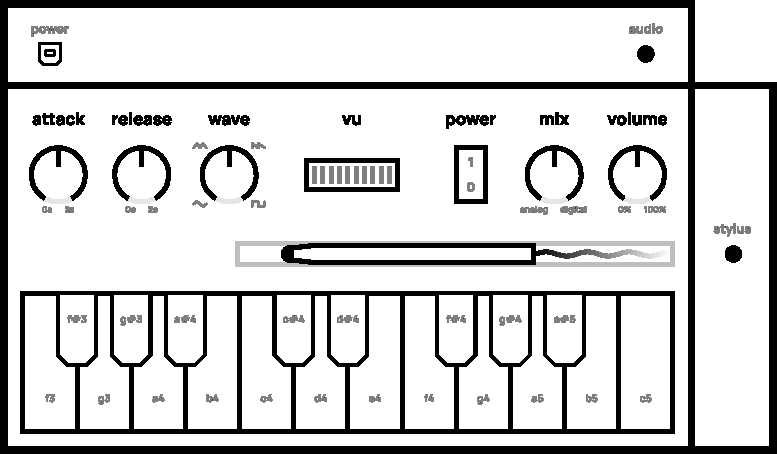
\includegraphics{figs/case-layout-sketch.pdf}
	\caption{Schets van de layout op de voor- en bovenkant}
\end{figure}

\section{Projectopdracht}

Hier is het originele verhaal van de opdrachtgever, met toegevoegde nummers om aan te
tonen hoe bepaalde eisen verwerkt zijn:

``Ik wil graag één muziekinstrument\req{20keys} die op twee verschillende manieren
geluid kan produceren\req{engines}, met een Stylofoon en Synthesizer. De Stylofoon
moet 20 tonen kunnen genereren\req{20keys}. De Synthesizer moet gebaseerd zijn op een
Arduino\req{engines} en 8 variabele tonen maken\req{readtone}\up{,}\req{wavform}. De
tonen die de Synthesizer maakt moeten met draaiknoppen instelbaar zijn op
frequentie\req{tuneable} en lengte\req{release}. Er moet een schakelaar aanwezig zijn
om te wisselen tussen het afspelen van de Stylofoon en Synthesizer\req{mixfader}. Het
geluidsignaal moet ook visueel gemaakt worden op een VU-meter\req{vumeter}. Het
volume moet ingesteld kunnen worden met een draaiknop\req{volknob}. De status van het
gehele instrument moet visueel weergegeven worden\req{powerbutton}. Het zou mooi zijn
als in plaats van een schakelaar er een manier is om de geluidssignalen van de
Stylofoon en Synthesizer te combineren\req{mixfader}.

De Stylofoon heeft minimaal 20 contactpunten\req{20keys} en is gebaseerd op een 555
timer\req{555}. De Synthesizer is gebaseerd op een Arduino Uno\req{engines} en heeft
minimaal 8 druktoetsen\req{readtone} en 2
draaiknoppen\req{digsoundtweak}. Verder is er een draaiknop om het
volume te regelen\req{volknob}, een luidspreker-aansluiting\req{phonesout} en een
VU-meter\req{vumeter}. Alleen pinnen A0-A5 van de Arduino Uno mogen gebruikt
worden\req{a05}.''

\section{Technische eisen}

In deze vereisten word er met het woord `synthesizer' alleen het elektrische
onderdeel dat een geluidssignaal produceert bedoeld, niet de stylofoon in zijn
geheel.

\begin{enumerate}
\subsection{Functionele specificaties}
	\item \label{req:20keys} \'E\'en fysiek klaviertoetsenbord bestaand uit 20
		elektrisch geleidende contacten
	\item \label{req:mixfader} Een draaiknop die het geluid van de analoge en de
		digitale synthesizers mixt voordat het signaal versterkt wordt
	\item \label{req:vumeter} Een 10-segments VU-meter die visueel de amplitude van het
		uigangssignaal laat zien
	\item \label{req:volknob} Een volumeknop om het uigangsvolume aan te passen
	\item \label{req:powerbutton} Een aan-uit knop op de voorkant die toont of de stylofoon
		aan staat
	\item \label{req:digsoundtweak} Draaiknoppen om eigenschappen van het geluid dat
		uit de digitale synthesizer komt aan te passen:
	\begin{enumerate}
		\item \label{req:attack} \'E\'en draaiknop om de attacktijd te regelen
		\item \label{req:release} \'E\'en draaiknop om de releasetijd te regelen
		\item \label{req:wavform} \'E\'en draaiknop om de golfvorm te mengen of schakelen
			tussen een sinus-, driehoeks-, zaagtand- en blokgolf.
	\end{enumerate}
\subsection{Operationele functies}
	\item \label{req:tuneable} De individuele tonen van de analoge synthesizer zijn
		stembaar met behulp van instelpotmeters
	\item \label{req:engines} Twee synthesizers, een analoge en een digitale die met
		behulp van een Arduino Uno gemaakt wordt
	\begin{enumerate}
		\item \label{req:wavforms} De digitale synthesizer produceert vier verschillende
			golfvormen
		\item \label{req:readtone} De digitale synthesizer kan de huidige toon die
			gespeeld word uitlezen door de spanning over de weerstandsladder te meten
	\end{enumerate}
	\item \label{req:phonesout} De audio uitgang van de stylofoon wordt intern
		versterkt zijn om op headphone-level te komen
\subsection{Ontwerpbeperkingen}
	\item \label{req:555} De analoge synthesizer is gebaseerd op een 555 timer
	\item \label{req:a05} Alleen pinnen A0..A5 van de Arduino worden gebruikt
	\item \label{req:lm3914} Er wordt een LM3914 IC gebruikt voor de VU-meter
\subsection{Randvoorwaarden}
	\item Sommige componenten worden voorgeschreven
	\item Diverse componenten zoals de gaatjesprint, druktoetsen en leds worden door de
		labbeheerders geleverd
	\item Componenten die niet in voorraad zijn worden in overleg met de labbeheerders
		gekozen
	\item Er worden IC-voetjes gebruikt om de ledbar van de VU-meter, en andere IC's te
		monteren
\end{enumerate}

\end{document}

